\section{Scene Catalog and Controlled Two-View Ablation}
\label{app:construction}

\begin{figure*}[!t]
\centering
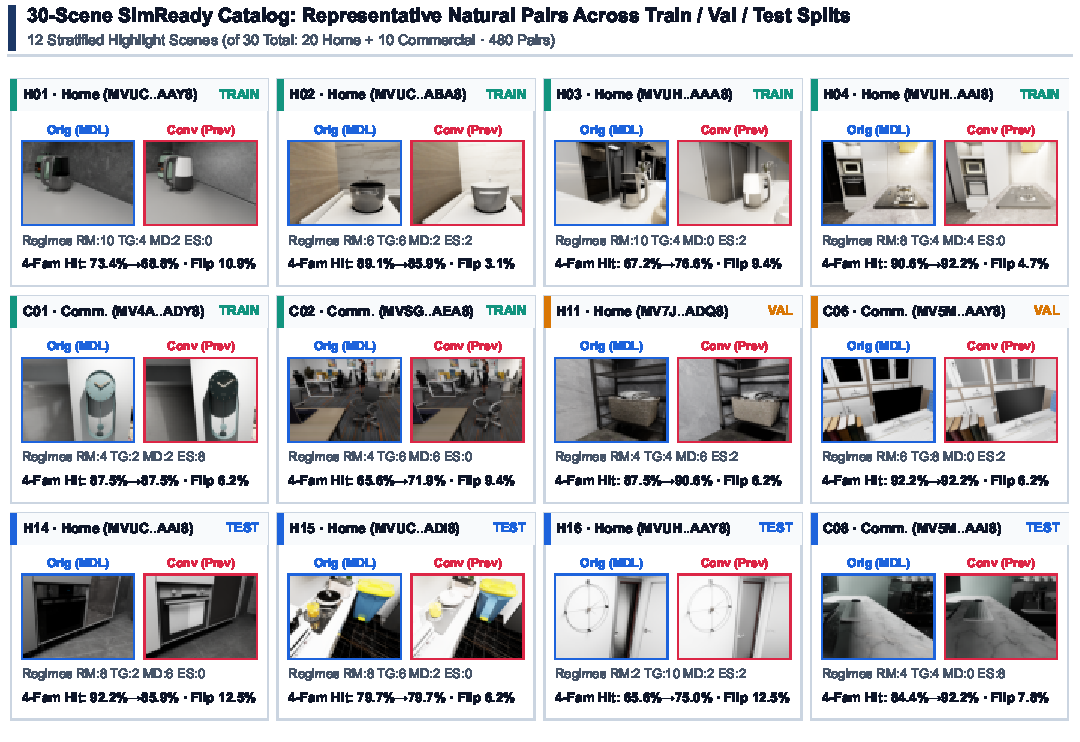
\includegraphics[width=0.94\textwidth]{app_fig2_scene30_atlas.pdf}
\caption{\textbf{Stratified catalog of the 30-scene \textsc{SimReady GRScenes} grounding benchmark.}
Twelve representative scenes spanning \texttt{Train} (15 scenes total), \texttt{Val} (5 scenes), and \texttt{Test} (10 scenes) across residential (\texttt{home\_scenes}, \texttt{H01--H20}) and commercial (\texttt{commercial\_scenes}, \texttt{C01--C10}) environments. Each card pairs canonical \original{} (\textsc{MDL}) and \converted{} (\usdps{}) captures, optical-regime composition (\texttt{RM/TG/MD/ES}), and four-family mean accuracy shift and decision flip rate; the full 30-scene breakdown appears in Table~\ref{tab:app-scenes30}.}
\label{fig:app-scene30}
\end{figure*}

\begin{table*}[!t]
\centering
\caption{Complete per-scene breakdown across all 30 independent \textsc{GRScenes} assets ($16$ camera pairs per scene; $480$ total pairs). Entries under each model report $H_O/H_C~(\mathrm{Flip\%})$ under deterministic greedy ($T{=}0$) evaluation; $\mathrm{SSIM}$ and $\Delta L^*$ report mean target-mask structural similarity and lightness shift.}
\label{tab:app-scenes30}
\resizebox{\textwidth}{!}{% Generated automatically by build_cviu_appendix_assets.py from pair_optical_features.json and v3 predictions
\begin{tabular}{@{}llllcrrrrrrr@{}}
\toprule
Code & Scene ID & Dom. & Split & RM/TG/MD/ES & SSIM & $\Delta L^*$ & Qwen3-8B & Qwen3-32B & InternVL3.5 & Molmo2-8B & LLaVA-7B \\
\midrule
H01 & \texttt{MVUC..AAY8} & Home & Train & 10/4/2/0 & 0.66 & 8.0 & 62/62 (12.5) & 81/81 (0.0) & 75/69 (6.2) & 100/100 (0.0) & 56/44 (25.0) \\
H02 & \texttt{MVUC..ABA8} & Home & Train & 6/6/2/2 & 0.66 & 10.6 & 88/88 (0.0) & 88/100 (12.5) & 88/81 (6.2) & 100/100 (0.0) & 81/75 (6.2) \\
H03 & \texttt{MVUH..AAA8} & Home & Train & 10/4/0/2 & 0.57 & 13.3 & 62/75 (12.5) & 88/81 (6.2) & 62/75 (12.5) & 94/94 (0.0) & 50/62 (12.5) \\
H04 & \texttt{MVUH..AAI8} & Home & Train & 8/4/4/0 & 0.73 & 5.4 & 94/94 (0.0) & 100/100 (0.0) & 81/88 (18.8) & 100/100 (0.0) & 88/88 (0.0) \\
H05 & \texttt{MVUH..AAI8} & Home & Train & 4/8/4/0 & 0.75 & 7.4 & 94/94 (12.5) & 94/94 (12.5) & 81/88 (6.2) & 88/100 (12.5) & 75/44 (31.2) \\
H06 & \texttt{MWAX..AAA8} & Home & Train & 10/4/2/0 & 0.56 & 13.4 & 81/88 (18.8) & 94/94 (0.0) & 81/88 (6.2) & 100/88 (12.5) & 56/56 (25.0) \\
H07 & \texttt{MWAX..ADA8} & Home & Train & 6/0/4/6 & 0.69 & 13.6 & 100/100 (0.0) & 100/100 (0.0) & 88/94 (6.2) & 88/88 (0.0) & 94/94 (0.0) \\
H08 & \texttt{MWAX..AEA8} & Home & Train & 8/2/6/0 & 0.74 & 9.8 & 100/100 (0.0) & 94/94 (0.0) & 75/75 (25.0) & 100/100 (0.0) & 81/81 (12.5) \\
H09 & \texttt{MWBG..ABA8} & Home & Train & 4/10/2/0 & 0.54 & 11.2 & 100/88 (12.5) & 100/100 (0.0) & 69/69 (12.5) & 94/100 (6.2) & 50/50 (12.5) \\
H10 & \texttt{MWBG..ABI8} & Home & Train & 4/2/6/4 & 0.73 & 15.5 & 81/88 (6.2) & 100/100 (0.0) & 88/94 (6.2) & 100/100 (0.0) & 62/69 (18.8) \\
C01 & \texttt{MV4A..ADY8} & Comm & Train & 4/2/2/8 & 0.65 & 7.1 & 88/94 (6.2) & 88/94 (6.2) & 88/88 (0.0) & 100/100 (0.0) & 75/69 (18.8) \\
C02 & \texttt{MVSG..AEA8} & Comm & Train & 4/6/6/0 & 0.74 & 4.9 & 50/56 (18.8) & 81/75 (6.2) & 75/81 (6.2) & 75/81 (6.2) & 62/69 (6.2) \\
C03 & \texttt{MWF4..ACI8} & Comm & Train & 4/12/0/0 & 0.71 & 8.9 & 75/81 (6.2) & 88/88 (0.0) & 81/81 (12.5) & 94/94 (0.0) & 88/88 (0.0) \\
C04 & \texttt{MWF4..ADI8} & Comm & Train & 0/6/2/8 & 0.63 & 10.2 & 69/69 (12.5) & 94/100 (6.2) & 69/75 (31.2) & 94/100 (6.2) & 50/62 (25.0) \\
C05 & \texttt{MWF4..ADQ8} & Comm & Train & 4/10/2/0 & 0.69 & 6.0 & 75/81 (6.2) & 75/81 (6.2) & 69/69 (12.5) & 94/100 (6.2) & 50/56 (56.2) \\
\midrule
H11 & \texttt{MV7J..ADQ8} & Home & Val & 4/4/6/2 & 0.71 & 6.9 & 94/94 (0.0) & 100/100 (0.0) & 94/100 (6.2) & 100/100 (0.0) & 62/69 (18.8) \\
H12 & \texttt{MV7J..ADY8} & Home & Val & 8/6/2/0 & 0.56 & 11.2 & 88/94 (6.2) & 100/100 (0.0) & 94/94 (12.5) & 100/100 (0.0) & 75/81 (18.8) \\
H13 & \texttt{MV7J..AEA8} & Home & Val & 2/8/2/4 & 0.52 & 17.5 & 94/88 (18.8) & 100/100 (0.0) & 88/88 (25.0) & 88/88 (12.5) & 75/62 (37.5) \\
C06 & \texttt{MV5M..AAY8} & Comm & Val & 6/8/0/2 & 0.75 & 5.5 & 94/94 (12.5) & 100/100 (0.0) & 88/94 (6.2) & 100/100 (0.0) & 88/81 (6.2) \\
C07 & \texttt{MVSY..ACY8} & Comm & Val & 4/4/6/2 & 0.66 & 3.3 & 62/69 (18.8) & 69/81 (12.5) & 56/62 (6.2) & 75/75 (25.0) & 50/56 (31.2) \\
\midrule
H14 & \texttt{MVUC..AAI8} & Home & Test & 8/2/6/0 & 0.61 & 11.8 & 94/88 (18.8) & 94/100 (6.2) & 94/81 (12.5) & 100/88 (12.5) & 81/88 (6.2) \\
H15 & \texttt{MVUC..ADI8} & Home & Test & 8/6/2/0 & 0.65 & 14.0 & 75/81 (6.2) & 100/94 (6.2) & 75/69 (6.2) & 100/100 (0.0) & 69/69 (12.5) \\
H16 & \texttt{MVUH..AAY8} & Home & Test & 2/10/2/2 & 0.64 & 5.3 & 69/75 (18.8) & 94/88 (6.2) & 62/69 (6.2) & 88/88 (0.0) & 44/69 (25.0) \\
H17 & \texttt{MVUH..ACQ8} & Home & Test & 4/6/4/2 & 0.47 & 5.4 & 62/75 (12.5) & 88/81 (6.2) & 69/62 (31.2) & 100/94 (6.2) & 31/38 (18.8) \\
H18 & \texttt{MVUH..ADA8} & Home & Test & 4/10/2/0 & 0.58 & 10.8 & 100/100 (0.0) & 94/94 (0.0) & 94/88 (6.2) & 100/100 (0.0) & 81/75 (18.8) \\
H19 & \texttt{MWAX..ADQ8} & Home & Test & 2/10/4/0 & 0.65 & 6.3 & 81/81 (12.5) & 100/100 (0.0) & 94/94 (0.0) & 100/100 (0.0) & 94/81 (12.5) \\
H20 & \texttt{MWBG..ACA8} & Home & Test & 6/4/4/2 & 0.60 & 17.1 & 81/81 (0.0) & 100/94 (6.2) & 75/75 (0.0) & 94/100 (6.2) & 50/56 (6.2) \\
C08 & \texttt{MV5M..AAI8} & Comm & Test & 4/4/0/8 & 0.76 & 2.7 & 75/88 (12.5) & 100/94 (6.2) & 75/81 (6.2) & 100/100 (0.0) & 88/100 (12.5) \\
C09 & \texttt{MWF4..ACY8} & Comm & Test & 2/12/2/0 & 0.59 & 6.4 & 94/88 (6.2) & 94/94 (0.0) & 81/81 (12.5) & 94/81 (12.5) & 56/50 (18.8) \\
C10 & \texttt{MWF4..AEA8} & Comm & Test & 8/2/2/4 & 0.60 & 8.0 & 56/44 (12.5) & 56/62 (18.8) & 50/50 (12.5) & 62/75 (12.5) & 62/56 (6.2) \\
\midrule
\textbf{All 30} & \textbf{480 pairs} & 20H/10C & 15/5/10 & \textbf{158/176/88/58} & \textbf{0.65} & \textbf{9.2} & \textbf{81.2/83.1 (9.4)} & \textbf{91.7/92.1 (4.2)} & \textbf{78.5/80.0 (10.6)} & \textbf{94.0/94.4 (4.6)} & \textbf{67.5/67.9 (16.7)} \\
\bottomrule
\end{tabular}
}
\end{table*}

\subsection{30-scene SimReady composition and mask integrity}
The 30-scene benchmark consists of \textbf{30 independent SimReady scenes} from \textsc{GRScenes} ($20$ residential \texttt{H01--H20} and $10$ commercial \texttt{C01--C10}), split at the scene level prior to feature fitting into \textbf{15 training (240 pairs), 5 validation (80 pairs), and 10 held-out test scenes (160 pairs)}. Within each scene, eight visible object instances are captured from two natural viewpoints at $1024{\times}768$, giving $240$ targets and $480$ paired captures ($960$ images), alongside three stratified control scenes ($48$ pairs) rendered across three independent path-tracing repeats under locked geometry and \textsc{MDL} materials. Figure~\ref{fig:app-scene30} depicts twelve representative scene cards, and Table~\ref{tab:app-scenes30} summarizes optical regimes and per-model turnover across all 30 scenes. Commercial scenes frequently match or exceed residential turnover across specialist and general models alike (e.g., \texttt{C10} flips $12.5\%$ even on \textsc{Molmo2-8B} and $18.8\%$ on \textsc{Qwen3-VL-32B}), indicating that shader-induced sensitivity extends well beyond domestic interiors.

\subsection{Controlled two-view gutter ablation}
\label{app:early_canvas}
In a supplementary controlled two-view ablation isolating four individual objects (bottle, clock, cup, and backpack), paired object captures were arranged cyclically across a 16-pixel neutral gray gutter on $(2W{+}16)\times H$ canvases in both left/right placements ($4{\times}2{\times}2 = 16$ queries per condition). Placing the frame midpoint inside the empty gutter rules out center-bias guessing, while target-window, context-window, and full-canvas crossovers built from integer bounding boxes motivate both the pixel-exact simulator masks $M_i^v$ and natural camera framing used in the main 30-scene benchmark.
